%% setup
\documentclass[multi=page]{standalone}
%
%% tikzipicture
\usepackage{tikz}
%
%% to use sans serif font
\renewcommand{\familydefault}{\sfdefault}
\usepackage{helvet}
% \usepackage{mathptmx} (times)


\begin{document}

%%%%%%%%%%%%%%
%% COMMANDS %%
%%%%%%%%%%%%%%

%% figurePage
%% goal: create a new figure page
% @arg1 - scaling of content of figure page
% @arg2 - content of figure page
\newcommand{\figurePage}[2]{
	\begin{page}
		\begin{tikzpicture}
			\node [minimum size = 18cm,rectangle,fill=white] at (0,0) {}; %% frame
			\node [scale=#1] at (0,0) {
				#2
			};
		\end{tikzpicture}
	\end{page}
}

%% cropMask
%% goal: create a crop mask function
% @arg1 - width of mask
% @arg2 - height of mask
% @arg3 - x center of mask content
% @arg4 - y center of mask content
% @arg5 - x position of mask 
% @arg6 - y position of mask
% @arg7 - content of mask
\newcommand{\cropMask}[7]{
	\node [minimum width=#1,minimum height=#2,path picture={
			\node at (#3,#4) {
				#7
			};
		}] at (#5,#6) {};
}

%% drawSLP
%% goal: draw a SLP
\newcommand{\slp}[3]{
	\begin{tikzpicture}
		%
		\node [draw,circle,label={left:{#1}}] (R) at (-2.25,0.75) {};
	    \node [draw,circle,label={left:{#2}}] (N) at (-2.25,-1.25) {};
	    %
	    \node [draw,circle] (1) at (0,2) {};
	    \node [draw,circle] (2) at (0,1.5) {};
	    \node [draw,circle] (3) at (0,1) {};
	    \node [draw,circle] (4) at (0,.5) {};
	    \node [draw,circle] (5) at (0,0) {};
	    \node [draw,circle] (6) at (0,-.5) {};
	    \node [draw,circle] (7) at (0,-1) {};
	    \node [draw,circle] (8) at (0,-1.5) {};
	    \node [draw,circle] (9) at (0,-2) {};
	    \node [draw,circle] (10) at (0,-2.5) {};        
	    %
	    \node [draw,circle,label={right:{#3}}] (O) at (2.25,-0.25) {};
		%
		\draw [->,>=stealth] (N) to node[midway] {} (1);
		\draw [->,>=stealth] (R) to node[midway] {} (1);
		\draw [->,>=stealth] (N) to node[midway] {} (2);
		\draw [->,>=stealth] (R) to node[midway] {} (2);
		\draw [->,>=stealth] (N) to node[midway] {} (3);
		\draw [->,>=stealth] (R) to node[midway] {} (3);
		\draw [->,>=stealth] (N) to node[midway] {} (4);
		\draw [->,>=stealth] (R) to node[midway] {} (4);
		\draw [->,>=stealth] (N) to node[midway] {} (5);
		\draw [->,>=stealth] (R) to node[midway] {} (5);	
		\draw [->,>=stealth] (N) to node[midway] {} (6);
		\draw [->,>=stealth] (R) to node[midway] {} (6);
		\draw [->,>=stealth] (N) to node[midway] {} (7);
		\draw [->,>=stealth] (R) to node[midway] {} (7);
		\draw [->,>=stealth] (N) to node[midway] {} (8);
		\draw [->,>=stealth] (R) to node[midway] {} (8);
		\draw [->,>=stealth] (N) to node[midway] {} (9);
		\draw [->,>=stealth] (R) to node[midway] {} (9);
		\draw [->,>=stealth] (N) to node[midway] {} (10);
		\draw [->,>=stealth] (R) to node[midway] {} (10);		
		%
		\draw [->,>=stealth] (1) to node[midway] {} (O);
		\draw [->,>=stealth] (2) to node[midway] {} (O);
		\draw [->,>=stealth] (3) to node[midway] {} (O);
		\draw [->,>=stealth] (4) to node[midway] {} (O);
		\draw [->,>=stealth] (5) to node[midway] {} (O);
		\draw [->,>=stealth] (6) to node[midway] {} (O);
		\draw [->,>=stealth] (7) to node[midway] {} (O);
		\draw [->,>=stealth] (8) to node[midway] {} (O);
		\draw [->,>=stealth] (9) to node[midway] {} (O);
		\draw [->,>=stealth] (10) to node[midway] {} (O);	
		%		
	\end{tikzpicture}
}

%
%%%

%%%%%%%%%%%%%
%% FIGURES %%
%%%%%%%%%%%%%

% %% new figure
% \figurePage{0.9}{
% 	\begin{tikzpicture}[overlay]
% 		%
% 		%% SLP
% 		\node [] at (-4,3) {\slp{$X_1$}{$X_2$}{$\tilde{f}_1$}};
% 		\node [] at (-4,-3) {\slp{$X_1$}{$X_2$}{$\tilde{f}_2$}};
% 		%
% 		%% NODE predictions
% 		\node at (4,3)
% 		{
% 			\begin{tikzpicture}
% 				\draw [dashed] (0,0) .. controls (1,1) and (2,-2) .. (3,1);
% 				\draw[->,green,line width=2pt] (0,0) -- (1,1);
% 				\draw [fill=black] (0,0) circle (2pt);
% 				\draw [fill=black] (3,1) circle (2pt);
% 				\node at (0,-0.5) {$X_1$};
% 				\node at (1.25,1.25) {$\tilde{f}_1$};
% 				\draw [->,line width=2pt] (0,-2) -- (3,-2);
% 				\node at (0,-2.5) {$t_0$};
% 				\node at (3,-2.5) {$t_f$};
% 				\node at (4,1.5) {$X_1 + \int_{t_0}^{t_f} \tilde{f}_1 dt$};
% 			\end{tikzpicture}
% 		};
% 		%
% 		\node at (4,-3)
% 		{
% 			\begin{tikzpicture}
% 				\draw [dashed] (0,0) .. controls (1,-1) and (2,2) .. (3,1);
% 				\draw[->,red,line width=2pt] (0,0) -- (1,-1);
% 				\draw [fill=black] (0,0) circle (2pt);
% 				\draw [fill=black] (3,1) circle (2pt);
% 				\node at (0,0.5) {$X_2$};
% 				\node at (1.25,-1.25) {$\tilde{f}_2$};
% 				\draw [->,line width=2pt] (0,-2) -- (3,-2);
% 				\node at (0,-2.5) {$t_0$};
% 				\node at (3,-2.5) {$t_f$};
% 				\node at (4,1.5) {$X_2 + \int_{t_0}^{t_f} \tilde{f}_2 dt$};
% 			\end{tikzpicture}
% 		};
% 		%
% 	\end{tikzpicture}
% }

%% new figure
\figurePage{0.9}{
	\begin{tikzpicture}[overlay]
	%
		\def\hspread{6}
		\def\vspread{3.7}
		\node [] at (-\hspread,0)  {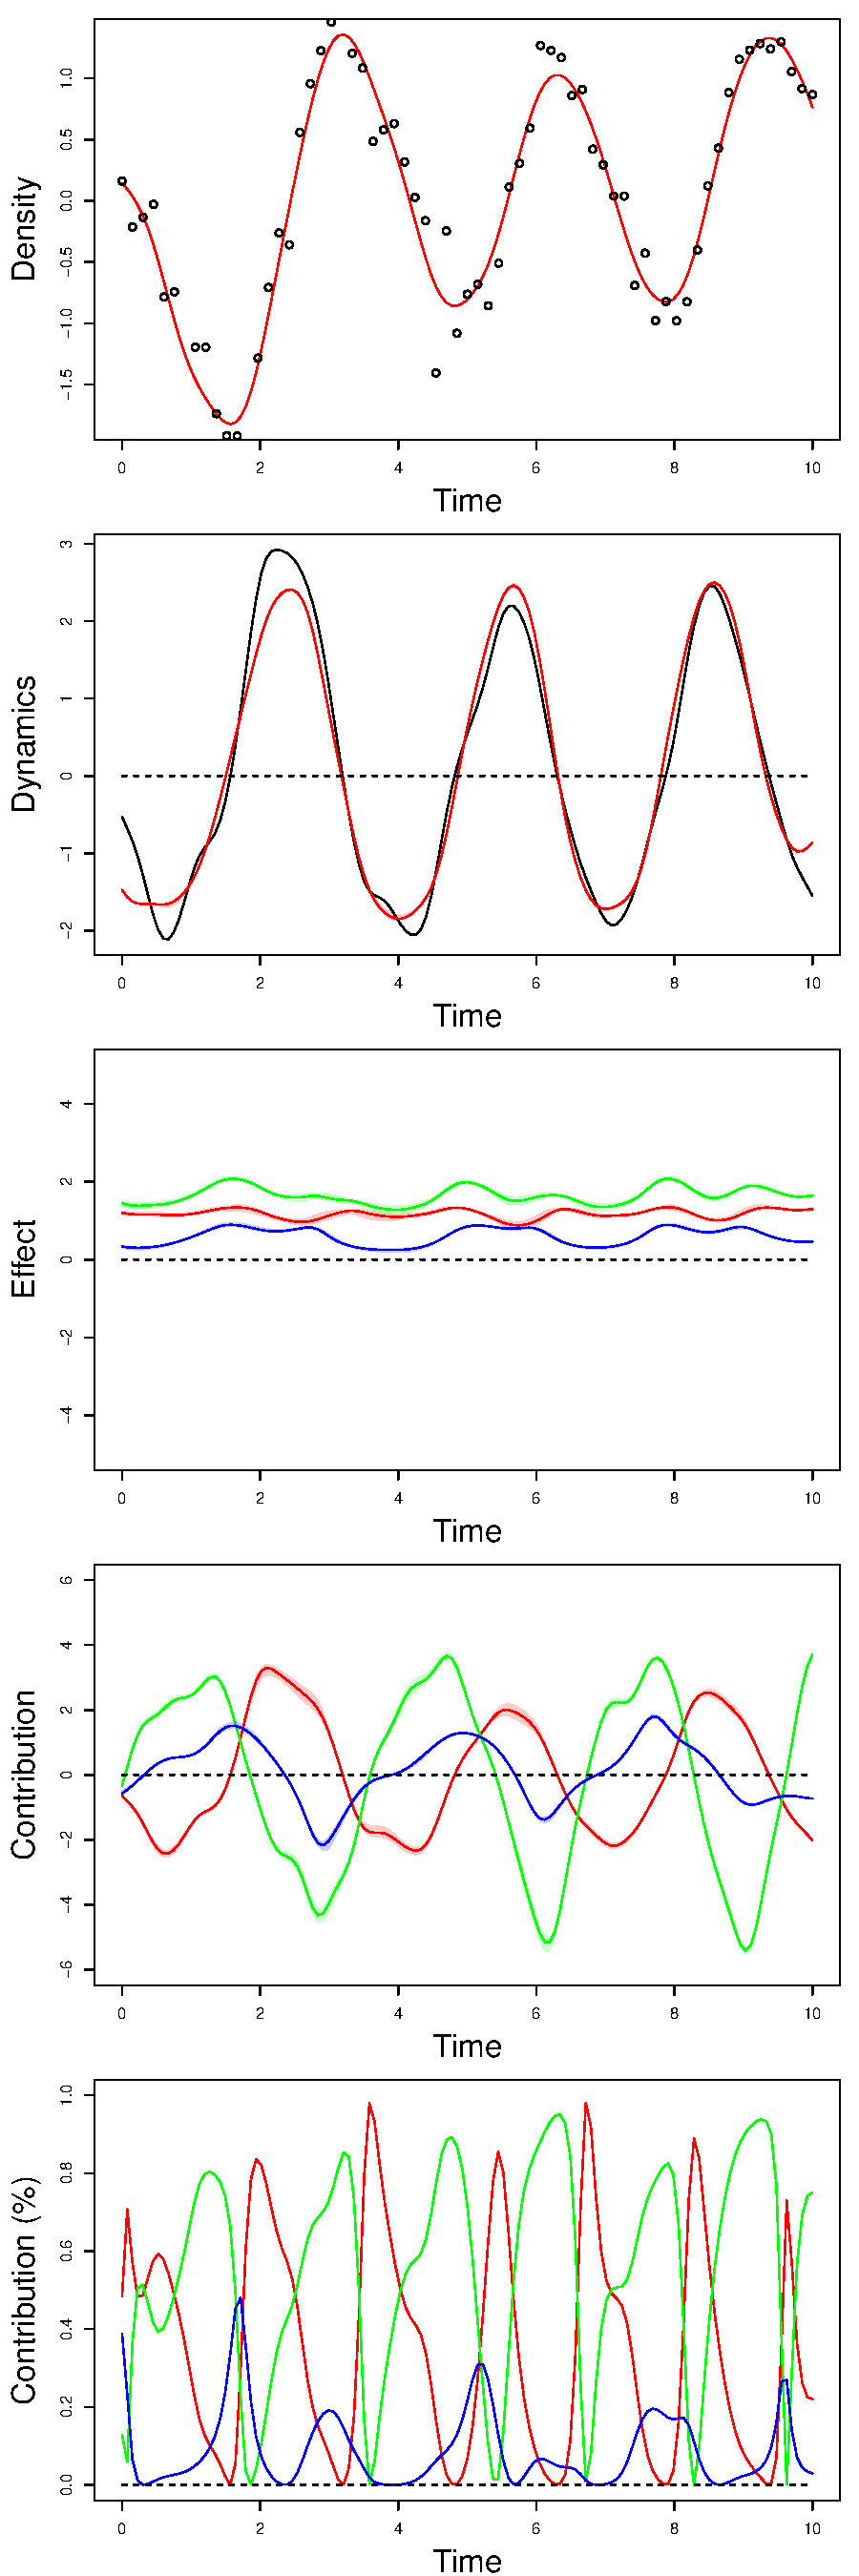
\includegraphics[page=1,width=6cm]{supporting/TS_analysis_1.pdf}};
		\node [] at (0,0)          {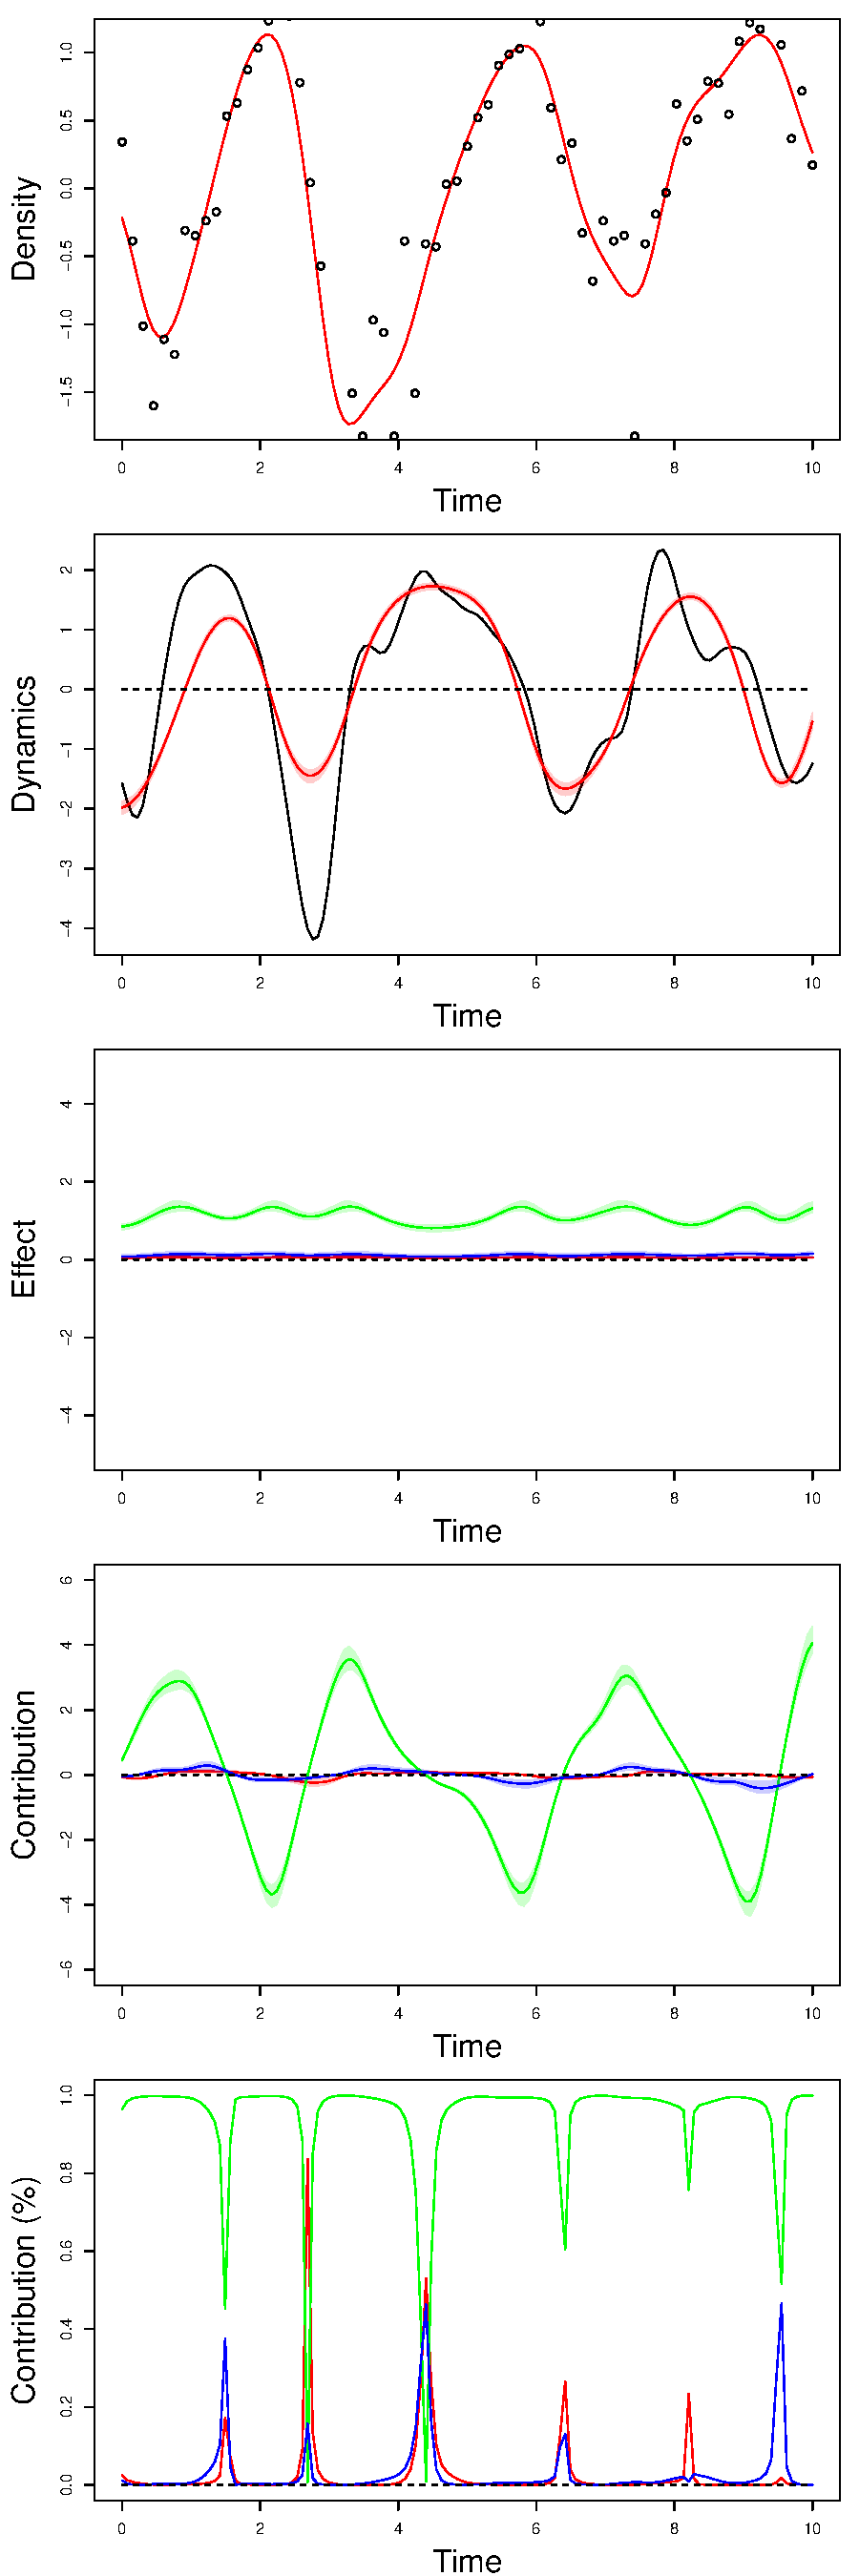
\includegraphics[page=1,width=6cm]{supporting/TS_analysis_2.pdf}};
		\node [] at (\hspread,0)   {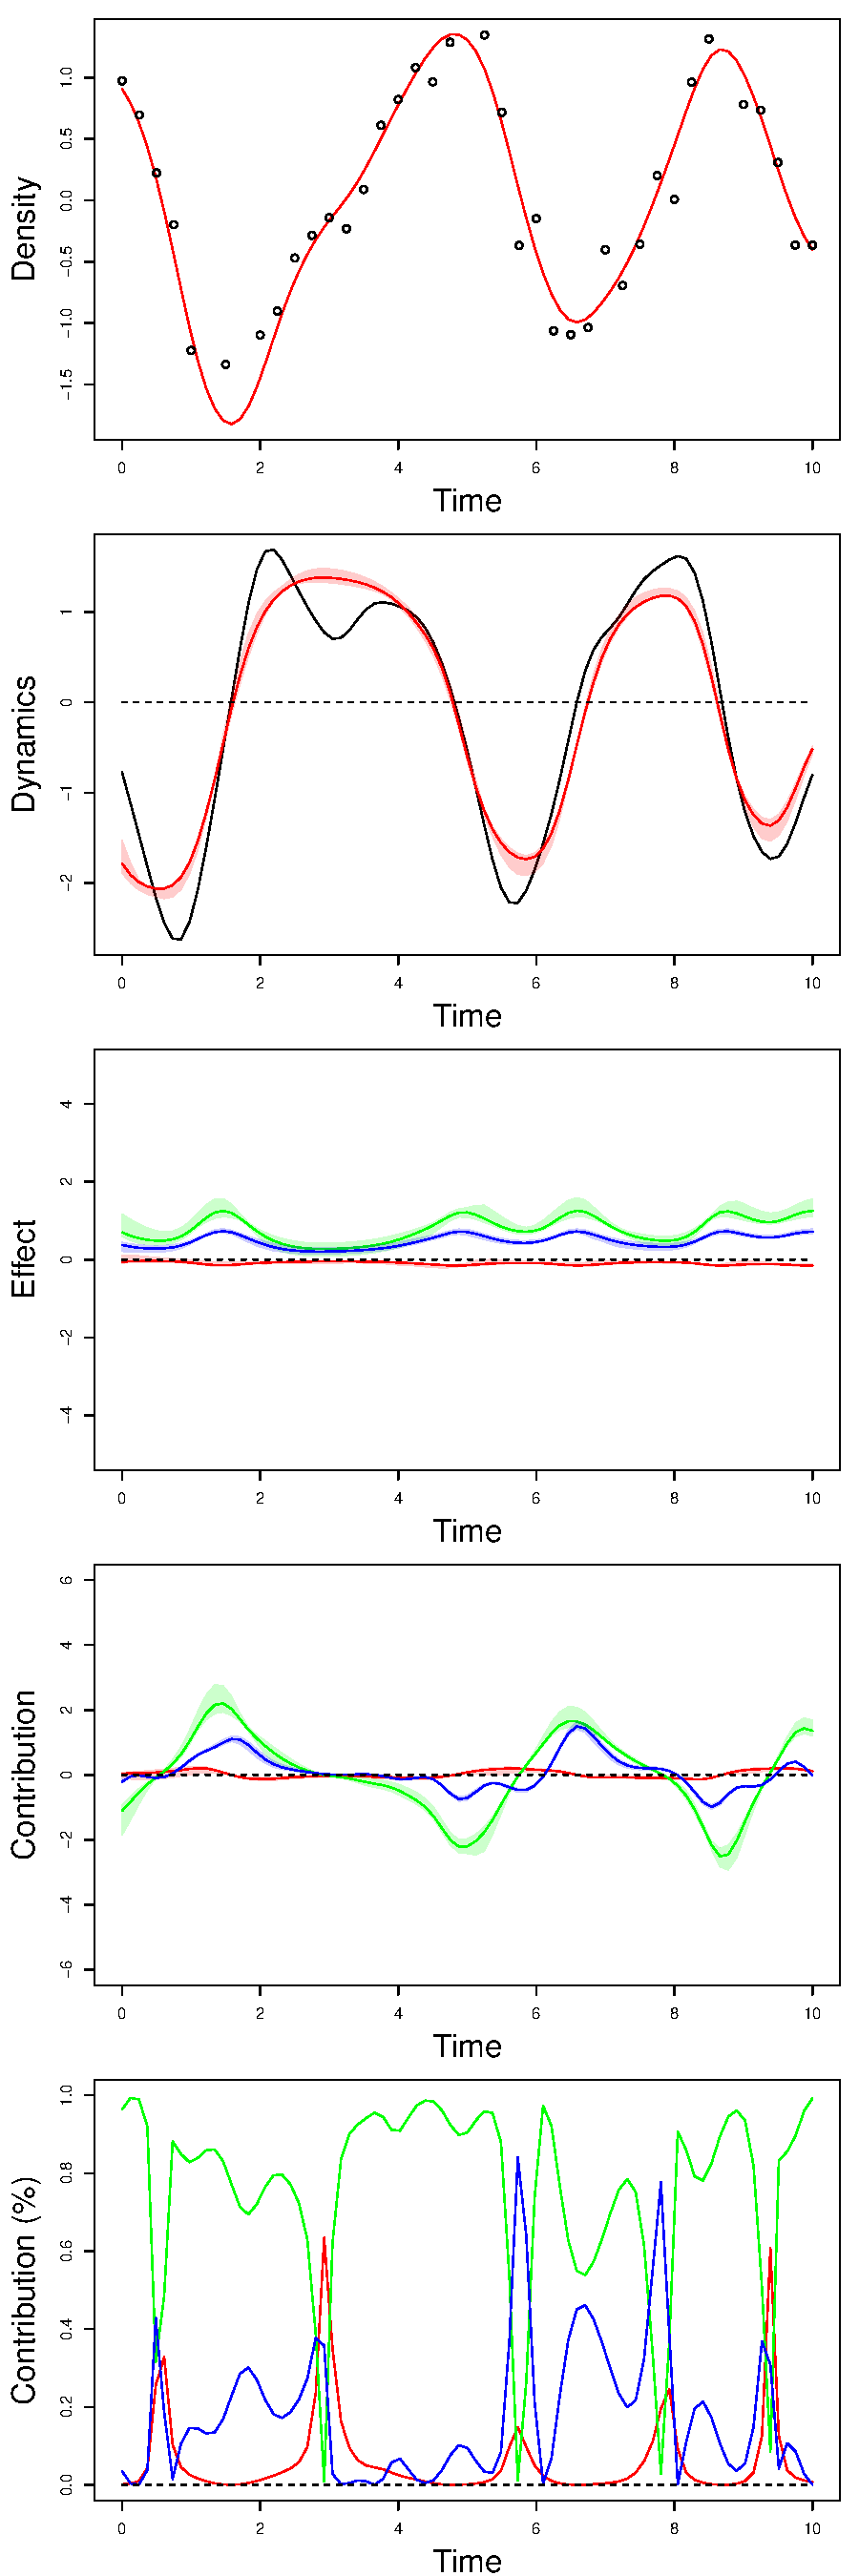
\includegraphics[page=1,width=6cm]{supporting/TS_analysis_3.pdf}};
		%
		%% legend
		\node [] at (-\hspread,9.5) {\textbf{Replicate A}};
		\node [] at (0,9.5)         {\textbf{Replicate B}};
		\node [] at (\hspread,9.5)  {\textbf{Replicate C}};
	    \node [] at (-\hspread-3.5,0+2*\vspread) {\textbf{1}};
	    \node [] at (-\hspread-3.5,0+1*\vspread) {\textbf{2}};
	    \node [] at (-\hspread-3.5,0+0*\vspread) {\textbf{3}};
	    \node [] at (-\hspread-3.5,0-1*\vspread) {\textbf{4}};
	    \node [] at (-\hspread-3.5,0-2*\vspread) {\textbf{5}};
	%
	\end{tikzpicture}
}

%% new figure
\figurePage{0.9}{
	\begin{tikzpicture}[overlay]
		\def\hspread{6}
		\def\vspread{3.7}
		\node [] at (-\hspread,0)  {\includegraphics[page=2,width=6cm]{supporting/TS_analysis_1.pdf}};
		\node [] at (0,0)          {\includegraphics[page=2,width=6cm]{supporting/TS_analysis_2.pdf}};
		\node [] at (\hspread,0)   {\includegraphics[page=2,width=6cm]{supporting/TS_analysis_3.pdf}};
		%% legend
		\node [] at (-\hspread,9.5) {\textbf{Replicate A}};
		\node [] at (0,9.5)         {\textbf{Replicate B}};
		\node [] at (\hspread,9.5)  {\textbf{Replicate C}};
	    \node [] at (-\hspread-3.5,0+2*\vspread) {\textbf{1}};
	    \node [] at (-\hspread-3.5,0+1*\vspread) {\textbf{2}};
	    \node [] at (-\hspread-3.5,0+0*\vspread) {\textbf{3}};
	    \node [] at (-\hspread-3.5,0-1*\vspread) {\textbf{4}};
	    \node [] at (-\hspread-3.5,0-2*\vspread) {\textbf{5}};
	\end{tikzpicture}
}

%% new figure
\figurePage{0.9}{
	\begin{tikzpicture}[overlay]
		\def\hspread{6}
		\def\vspread{3.7}
		\node [] at (-\hspread,0)  {\includegraphics[page=3,width=6cm]{supporting/TS_analysis_1.pdf}};
		\node [] at (0,0)          {\includegraphics[page=3,width=6cm]{supporting/TS_analysis_2.pdf}};
		\node [] at (\hspread,0)   {\includegraphics[page=3,width=6cm]{supporting/TS_analysis_3.pdf}};
		%
		%% legend
		\node [] at (-\hspread,9.5) {\textbf{Replicate A}};
		\node [] at (0,9.5)         {\textbf{Replicate B}};
		\node [] at (\hspread,9.5)  {\textbf{Replicate C}};
	    \node [] at (-\hspread-3.5,0+2*\vspread) {\textbf{1}};
	    \node [] at (-\hspread-3.5,0+1*\vspread) {\textbf{2}};
	    \node [] at (-\hspread-3.5,0+0*\vspread) {\textbf{3}};
	    \node [] at (-\hspread-3.5,0-1*\vspread) {\textbf{4}};
	    \node [] at (-\hspread-3.5,0-2*\vspread) {\textbf{5}};
	%
	\end{tikzpicture}
}

%% new figure
\figurePage{0.9}{
	\begin{tikzpicture}[overlay]
	%
		\def\hspread{6}
		\node [] at (\hspread,0)  {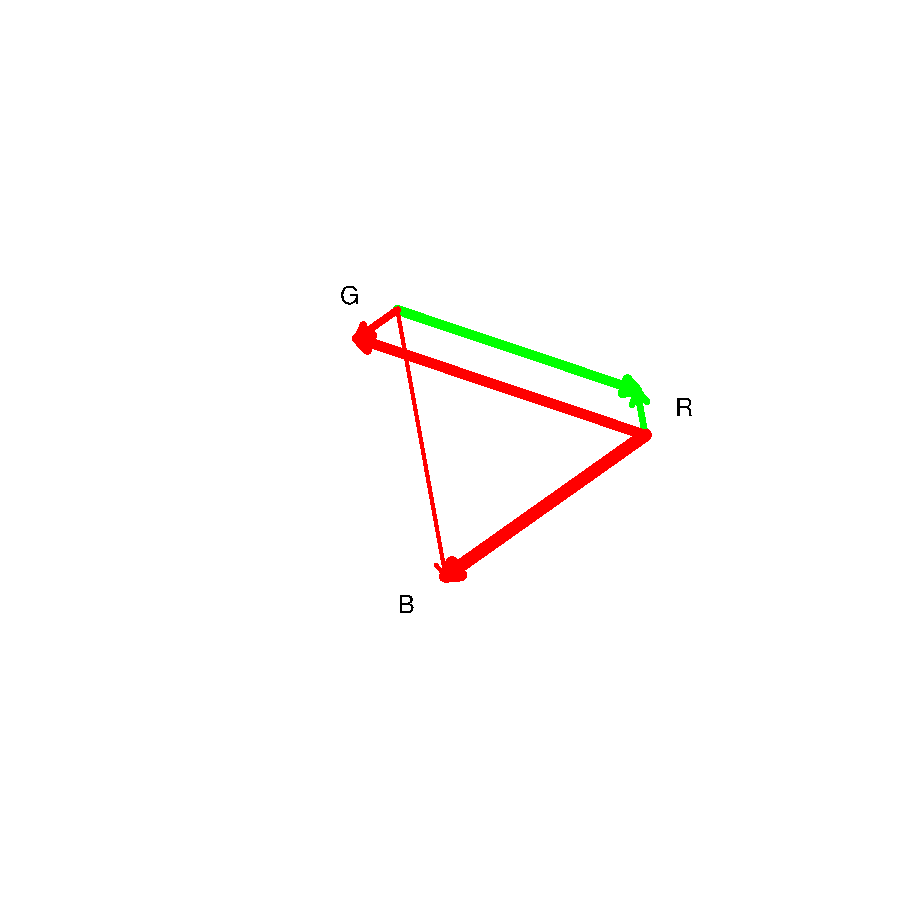
\includegraphics[height=6cm,width=6cm]{supporting/TS_DIN_1.pdf}};
		\node [] at (0,0)         {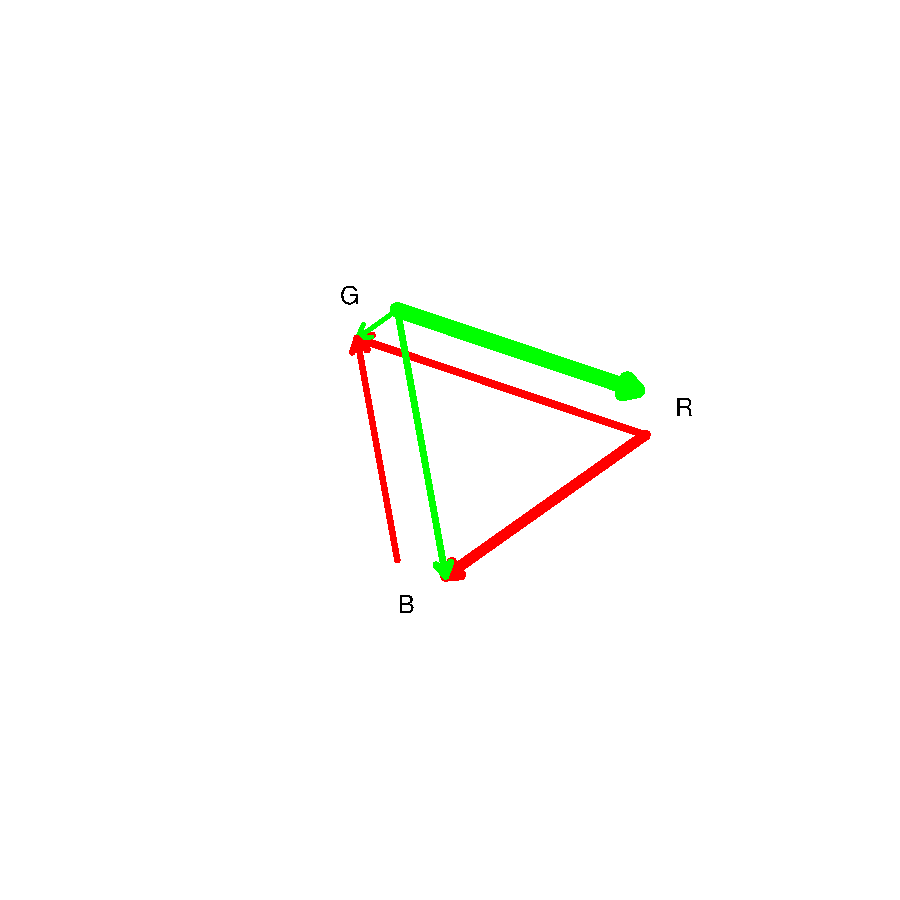
\includegraphics[height=6cm,width=6cm]{supporting/TS_DIN_2.pdf}};
		\node [] at (-\hspread,0) {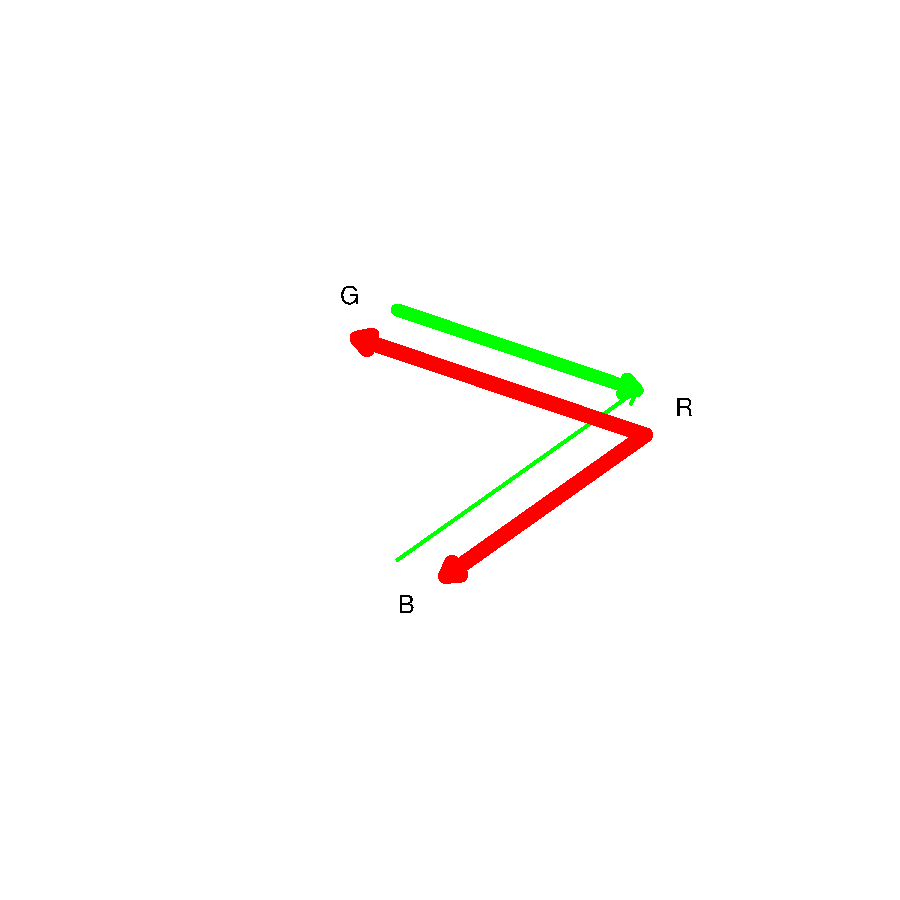
\includegraphics[height=6cm,width=6cm]{supporting/TS_DIN_3.pdf}};
		%
		%% legend
		\node [] at (-\hspread,3) {\textbf{Replicate A}};
		\node [] at (0,        3) {\textbf{Replicate B}};
		\node [] at (\hspread, 3)  {\textbf{Replicate C}};
	%
	\end{tikzpicture}
}

\end{document}
